\section{Project 9 - Image Segmentation}

\subsection{Project Proposal}
There tow parts of project 9. One task is for edge detection: implement the Roberts, Prewitt, Sobel, the Marr-Hildreth and the Canny edge detectors. The test image is \emph{building.tif}. The other task is to implement the Otsu’s method of thresholding segmentation, and compare the results with the global thresholding method using test image \emph{polymersomes.tif}.

\subsection{Preliminaries}
\subsubsection{Edge detection}
The central idea of edge detection is that local changes in intensity can be detected using derivatives. We have the following conclusions which show that first- and second-order derivatives are particularly well suited for this purpose: (1) First-order derivatives generally produce thicker edges in an image. (2) Second-order derivatives have a stronger response to fine details such as thin lines, isolated points, and noise. (3) Second-order derivatives produce a double-edge response at ramp and step transitions in intensity. (4) The sign of the second derivative can be used to determine whether a transition into an edge is from light to dark or dark to light.

\subsubsection{Basic edge detection}
The tool of choice for finding edge strength and direction at location $(x, y)$ of an image $f$ is the gradient. 
\begin{equation} \nabla f \equiv \text{grad}(f) \equiv \left[ \begin{array}{c} g_x \\ g_y \end{array}\right] = \left[ \begin{array}{c} \frac{\partial f}{\partial x} \\ \frac{\partial f}{\partial y} \end{array} \right] 
\end{equation}
The magnitude of vector $\nabla f$ defined as \begin{equation} \label{eq:magnitude} M(x,y)=mag(\nabla f) =  \sqrt{g_x^2 + g_y^2} \approx |g_x| + |g_y| \end{equation} is the value of the rate of change in the direction of the gradient vector. The second $=$ is a frequently used approximate to avoid square roots. The direction of gradient vector is given by the angle \begin{equation} \alpha(x,y)=\tan^{-1} \left[ \frac{g_y}{g_x} \right] \label{eq:angle} \end{equation}
The direction of an edge at an arbitrary point $(x,y)$ is orthogonal to the direction $\alpha(x,y)$. 
Here we mention three masks(Figure \ref{fig:3masks}) Roberts, Prewitt and Sobel which can be used to compute the gradient of the center point with convolution operation.
\begin{figure}[h!]
	\centering
	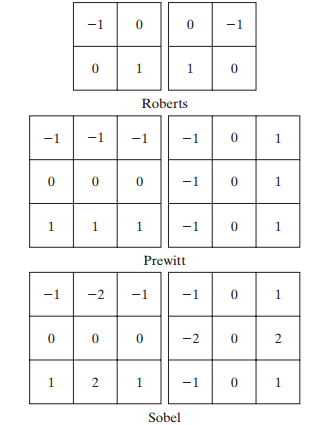
\includegraphics[scale=0.7]{myfigure/p9/3masks.png}
	\caption{3 masks for gradient computation: Roberts, Prewitt, Sobel}
	\label{fig:3masks}
\end{figure}

\subsubsection{More advanced techniques for edge detection}
\textbf{The Marr-Hildreth edge detector} is able to compute the approximate numerical result of gradient operator for sharply focused detail as well as act at large scale to detect the blurry edges. This operator is defined as $\nabla^2 G$ where \begin{equation}G(x,y) = e^{-frac{x^2+y^2}{2\sigma^2}} \label{eq:gaussian_2}\end{equation}. Then the so-called \emph{Laplacian of Gaussian(LoG)} is \begin{equation} \nabla^2 G(x,y) = \left[ \frac{x^2+y^2-\sigma^2}{4\sigma^4} \right]e^{-\frac{x^2+y^2}{2\sigma^2}} \end{equation} The use of LoG filter can be represented as \begin{equation} g(x,y)=\nabla^2\left[G(x,y)\right]\circ f(x,y) \end{equation}. Because of linear process, we can also write it as \begin{equation} g(x,y)=\nabla^2\left[G(x,y)\circ f(x,y)\right] \end{equation} 
Hence, the steps of Marr-Hildreth algorithm can be summarized as: \textbf{1.}Filter the input image with $n\times n$ Gaussian lowpass filter obtained by sampling \ref{eq:gaussian_2}. \textbf{2.}Compute the Laplacian of the result of step \textbf{1} using, for example, $3\times 3$ mask. \textbf{3.}Find the zero crossing of the resulting image from step 2. \\
The method of finding zero crossing at any pixel $p$ is to use a $3\times 3$ neighborhood centered at $p$, if the absolute difference of any two opposite neighbors exceeds a given threshold, then $p$ is a zero-crossing pixel.\\
\\
\textbf{The Canny edge detector} is superior in general to all the detectors discussed before. The algorithm consist the following steps: \\
\textbf{1.}Smooth the input image with a Gaussian filter.\\ 
\textbf{2.}Compute the gradient magnitude $M(x,y)$ and angle $\alpha(x,y)$ images. \\
\textbf{3.}Apply nonmaxima suppression to the gradient magnitude image. \\
\textbf{4.}Use double thresholding and connectivity analysis to detect and link edge. \\
The first two steps are apparent as the definition in Eq.\ref{eq:magnitude} and Eq.\ref{eq:angle}. The step \textbf{3 nonmaxima suppression} is used to thin the coarse edges in magnitude image. The essence of nonmaxima suppression is to define a set of discrete orientation of the edge normal $\{ d_1, d_2, d_3, d_4 \}$, e.g. $0^\circ$, $45^\circ$, $90^\circ$, $-45^\circ$. To map edges of arbitrary direction to the discrete orientation, we define non-overlapping range for each given direction. We can formulate the nonmaxima suppression schema for a $3\times 3$ region centered at every point $(x,y)$ in angle image $\alpha(x,y)$: \\
\textbf{(1)}Find the direction $d_k$ that is closest to $\alpha(x,y)$. \\
\textbf{(2)}If the value of $M(x,y)$ is less than at least one of its two neighbor on this direction, let $g_N(x,y)=0$; otherwise, let $g_N(x,y)=M(x,y)$. \\
Then we come to step \textbf{4 double thresholding} on $g_N(x,y)$ to reduce the false edge points. In Canny's algorithm we use two thresholds, $T_L$ as the low threshold and $T_H$ as the high threshold. Canny suggests that the ratio of the high to low threshold should be two or three to one. The process of thresholding is, \begin{equation} g_{NH}(x,y)=g_N(x,y)\geq T_H \end{equation}\begin{equation} g_{NL}(x,y)=g_N(x,y)\geq T_L\end{equation} then eliminate all the nonzero pixels in $g_{NH}$ from $g_{NL}$ \begin{equation} g_{NL}(x,y) := g_{NL}(x,y)-g_{NH}(x,y) \end{equation} The pixels in $g_{NH}$ is viewed as strong valid edge pixels and are marked immediately, but there are many gaps on these edges that should be filled using information from $g_{NL}$. We do this by following these steps:\\
\textbf{(1)}Locate the next unvisited edge pixel $p$ in $g_{NH}$. \\
\textbf{(2)}Mark all the weak pixels in $g_{NL}$ that is 8-connective to $p$ as valid. \\
\textbf{(3)}If all nonzero pixels in $g_{NH}$ has been visited, goto step 4. Otherwise goto back to step 1. \\
\textbf{(4)}Set all the pixels that are not marked as valid in $g_{NL}$.\\
The final result of Canny's algorithm is formed by appending all the nonzero pixels in $g_{NL}$ to $g_{NH}$.
\subsubsection{Thresholding Segmentation}
Thresholding is useful in applications of image segmentation because of its simplicity of implementation and computational speed. We talk about the most basic intensity thresholding here. The basic formula is 
\begin{equation}g(x,y)=\left \{ \begin{array}{rcl}
1 & \text{if}f(x,y)>T \\
0 & \text{otherwise}  \end{array} \right.\label{eq:global_threshold}\end{equation}
When $T$ is a constant applicable over an entire image, the process given in this equation is referred to as \textbf{global thresholding}. \\
\\
\textbf{Basic global thresholding} algorithm is capable of estimate automatically the threshold value for each image is required. The following iterative algorithm can be used for this purpose:\\
\textbf{1.}Select an initial estimate for the global threshold $T$. Mean value of gray intensities is a good choice.\\
\textbf{2.}Segment the image using $T$ in Eq.\ref{eq:global_threshold}. This will result in two groups of pixels: $G_1$($g(x,y)>T$) and $G_2$($g(x,y)\leq T$)\\
\textbf{3.}Compute the average intensity values $m_1$ and $m_2$ for the two groups $G_1$ and $G_2$ respectively.\\
\textbf{4.}Compute a new threshold value: $T=(m_1+m_2)/2$\\
\textbf{5.}Repeat step2 through 4 until the difference between values of $T$ in successive iterations os smaller than a predefined parameter $\Delta T$.\\
Global thresholding seems very simple as we just need to select a proper value for $T$, but the problem is that, usually, we cannot directly find out such a $T$ that separates the hills in histogram. Noise in the image, illumination and reflectance and so on factors lead to this effect.
Then we discuss an attractive alternative \textbf{Otus's method} which is based entirely on computations performed on the histogram of an image. The algorithm can be summarized as follows:\\
\textbf{1.} Compute the normalized histogram of the input image. Denote the components of the histogram by $p_i, i=0,1,...,L-1$.\\
\textbf{2.} Compute the cumulative sums, $P_1(k)$, for $k=0,1,...,L-1$, using \begin{equation} P_1(k)=\sum_{i=0}^k p_i \end{equation}
\textbf{3.} Compute the cumulative means, $m(k)$, for $k=0,1,...,L-1$ using \begin{equation} m(k)=\sum_{i=0}^k ip_i\end{equation}
\textbf{4.} Compute the global intensity mean, $m_G$, using \begin{equation} m_G=\sum_{i=0}^{L-1}ip_i \end{equation}
\textbf{5.} Compute the between-class variance, $\sigma^2_B(k)$, for $k=0,1,...,L-1$ using \begin{equation} \sigma_B^2(k)=\frac{[m_GP_1(k)-m(k)]^2}{P_1(k)[1-P_1(k)]}\end{equation}
\textbf{6.} Obtain the Otsu threshold, $K^*$, as the value of $k$ for which $\sigma_B^2(k)$ is maximum. If the maximum is not unique, obtain $k^*$ by averaging the values of $k$ corresponding to the various maxima detected. \\
\textbf{7.} Obtain the separability measure, $\eta ^ *$, by at $k=k^*$ evaluating \begin{equation} \eta(k)=\frac{\sigma_B^2(k)}{\sigma_G^2}, \sigma_G^2=\sum_{i=0}^{L-1}(i-m_G)^2p_i \end{equation} 

\subsection{Experiment}
\subsubsection{Edge detection}
First, I display the basic method that only use derivative mask for convolution. These masks are \emph{Roberts, Prewitt and Sobel}. The results are shown in Fig.\ref{fig:basic_edge}. We can see that the result of Sobel and Prewitt is very similar while the result of Roberts is not as good as the two because of lower significance of edges.\\

\begin{figure}[h!]
	\centering
	\begin{subfigure}[b]{0.45\linewidth}
		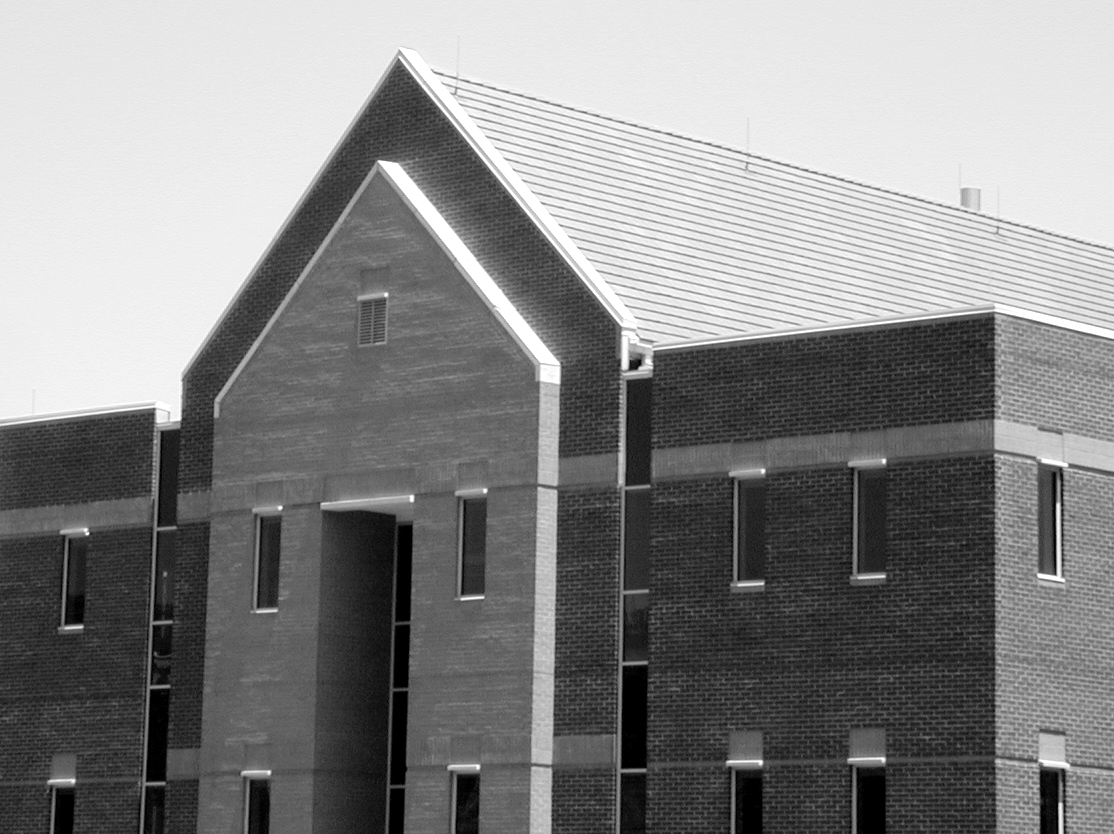
\includegraphics[width=\linewidth]{myfigure/p9/building.png}
		\caption{}
		\label{fig:basic_building}
	\end{subfigure}
	\begin{subfigure}[b]{0.45\linewidth}
    	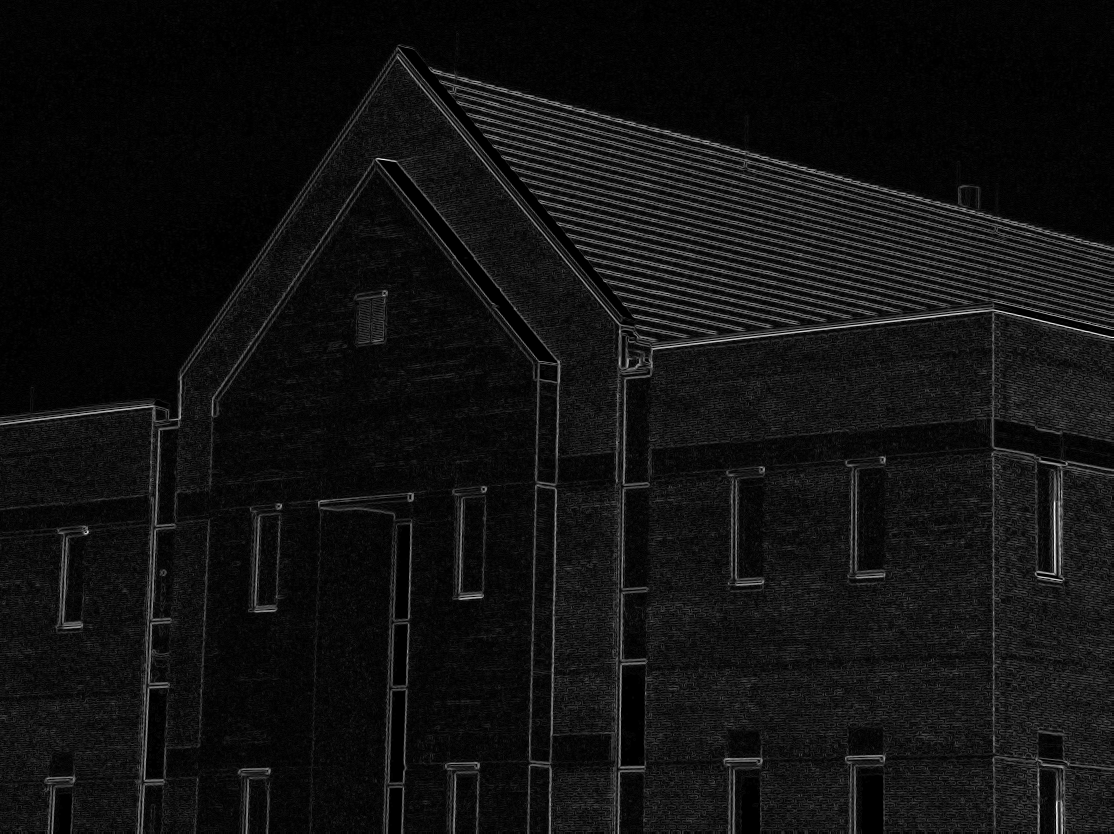
\includegraphics[width=\linewidth]{myfigure/p9/9_roberts.png}
    	\caption{}
    	\label{fig:roberts}
  	\end{subfigure}
  	\begin{subfigure}[b]{0.45\linewidth}
		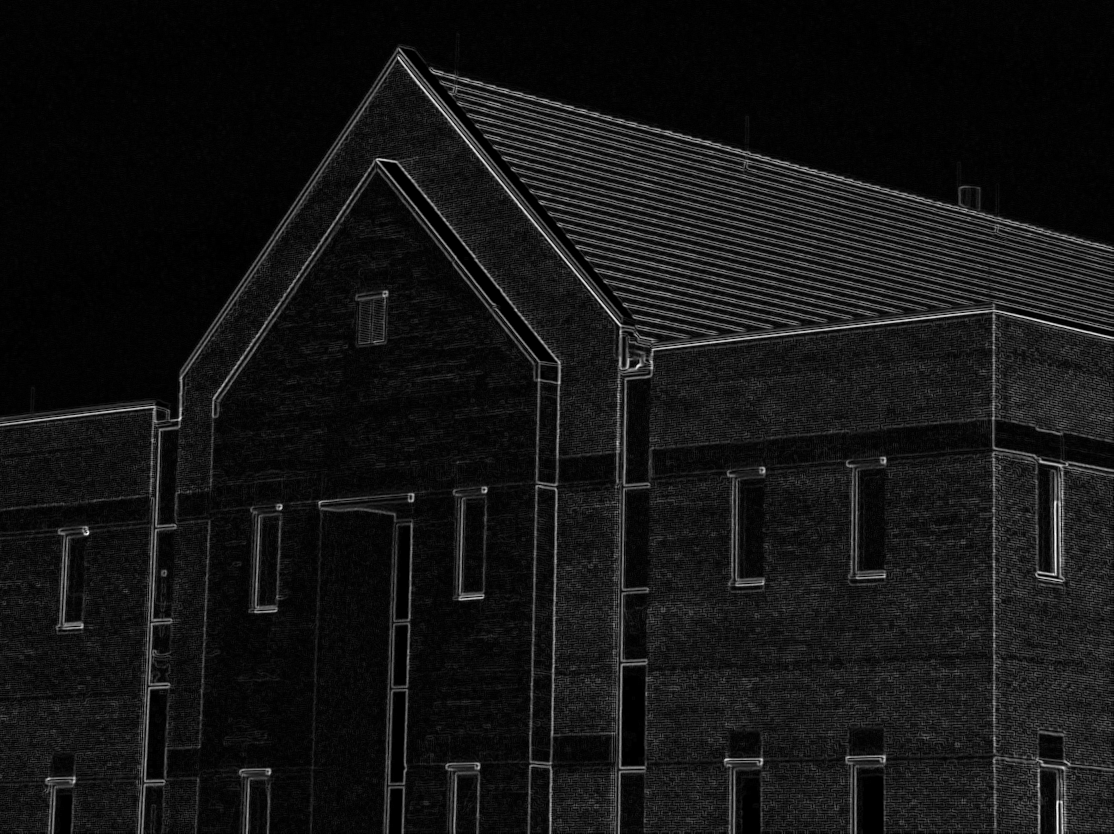
\includegraphics[width=\linewidth]{myfigure/p9/9_prewitt.png}
		\caption{}
		\label{fig:prewitt}
	\end{subfigure}
	\begin{subfigure}[b]{0.45\linewidth}
    	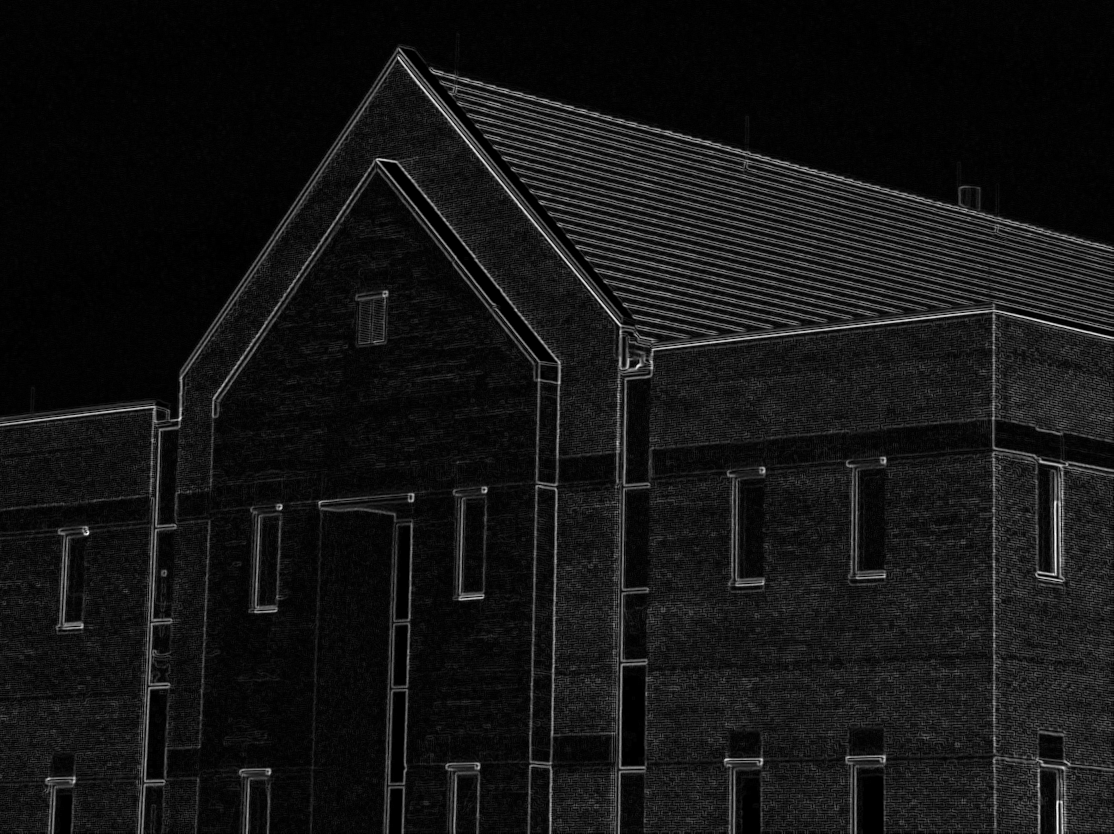
\includegraphics[width=\linewidth]{myfigure/p9/9_sobel.png}
    	\caption{}
    	\label{fig:sobel}
  	\end{subfigure}
  	\caption{Basic edge detection methods. (a)Original test image of size $834 \times 1115$. (b)Edge detection by Roberts mask. (c) Edge detection by Prewitt mask. (d)Edge detection by Sobel mask.}
  	\label{fig:basic_edge}
\end{figure}

Second, I show the process of applying Marr-Hildreth algorithm in Fig.\ref{fig:marr_hildreth}. In (c)-(d), we can see the effect of using threshold. I think that the use of Gaussian lowpass filter is a good idea for create margin between edge and other pixels. As there may be some trivial different between builtin function and self-defined function, the parameters used here is different from the ones given on the textbook. The size of Gaussian lowpass filter is $25\times 25$ and the variance is $\sigma=4$. After trying threshold as 0.04, 0.08, 0.12, I find $0.08$ is the best one.\\

\begin{figure}[h!]
	\centering
	\begin{subfigure}[b]{0.45\linewidth}
		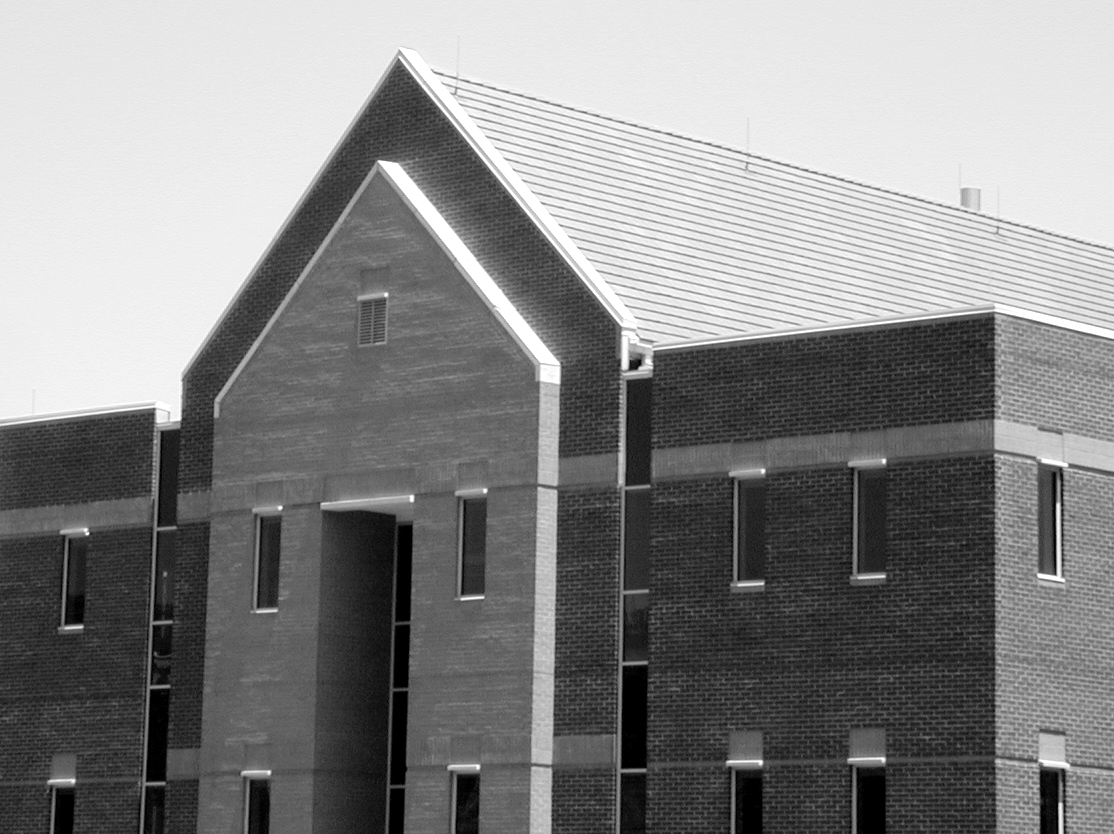
\includegraphics[width=\linewidth]{myfigure/p9/building.png}
		\caption{}
		\label{fig:marr_building}
	\end{subfigure}
	\begin{subfigure}[b]{0.45\linewidth}
    	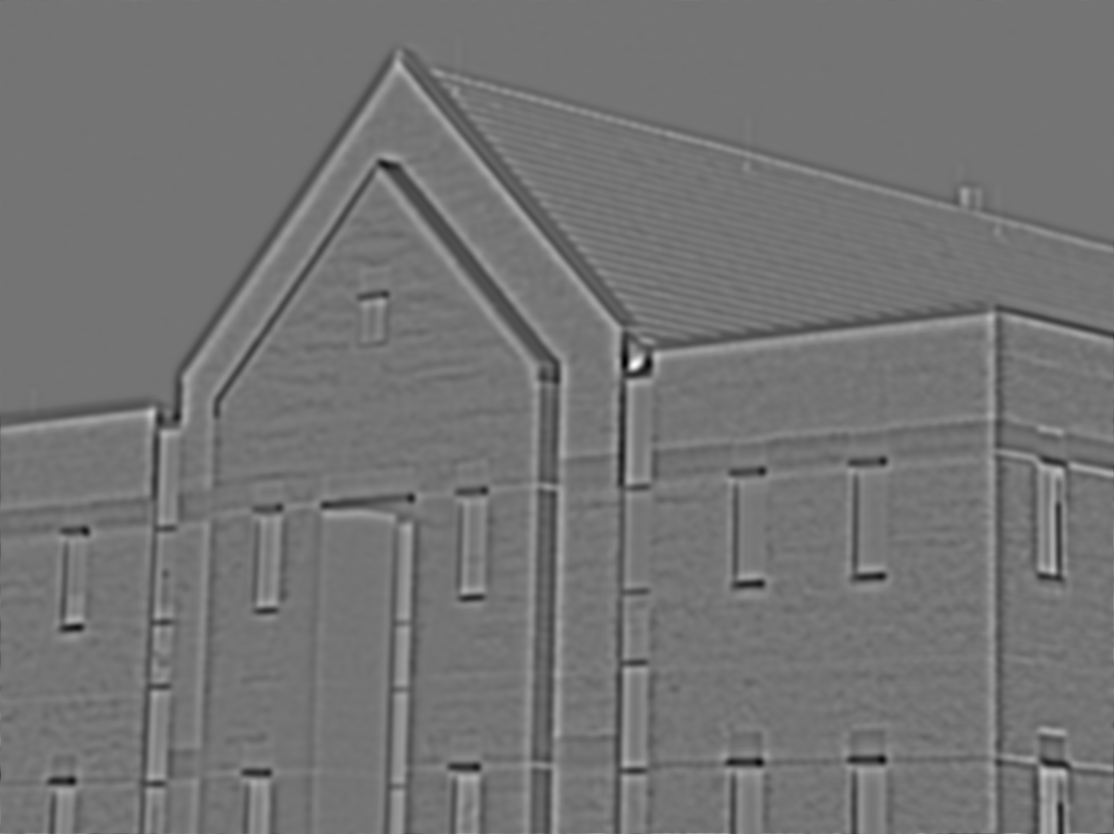
\includegraphics[width=\linewidth]{myfigure/p9/9_marrhildreth.png}
    	\caption{}
    	\label{fig:marrhildreth}
  	\end{subfigure}
  	\begin{subfigure}[b]{0.45\linewidth}
		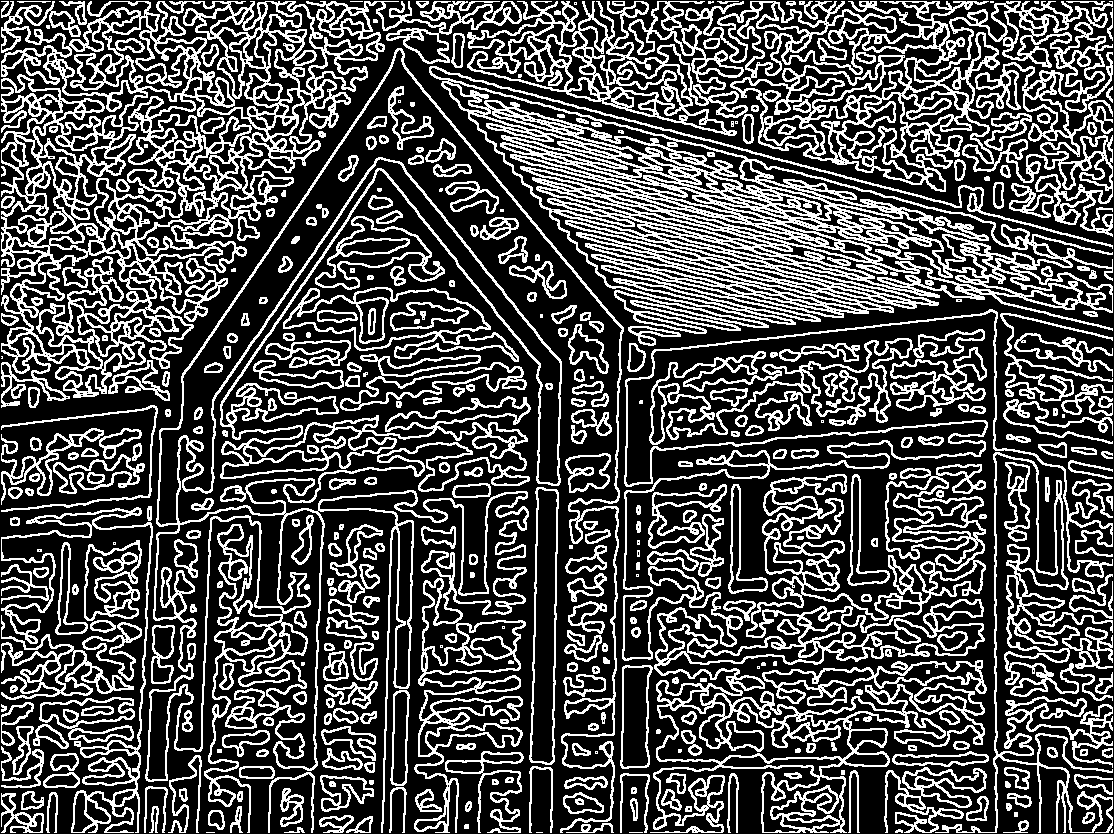
\includegraphics[width=\linewidth]{myfigure/p9/9_zerocross_0.png}
		\caption{}
		\label{fig:zerocross_0}
	\end{subfigure}
	\begin{subfigure}[b]{0.45\linewidth}
		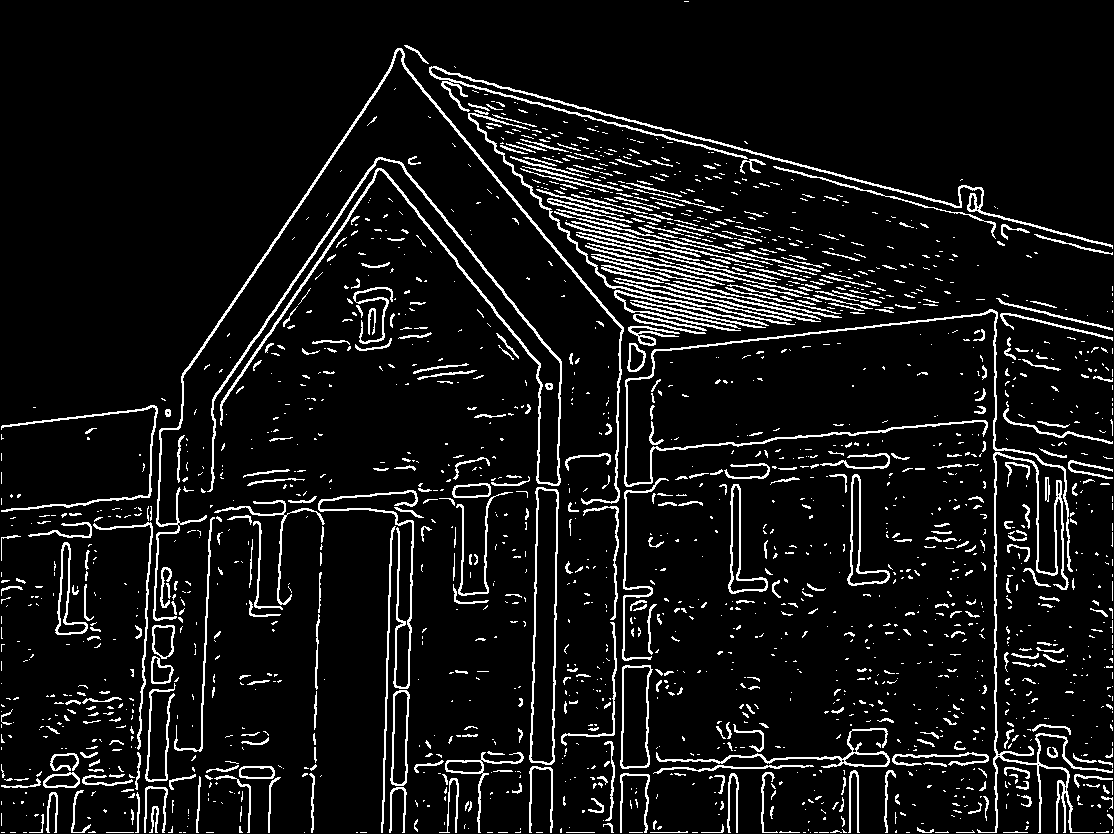
\includegraphics[width=\linewidth]{myfigure/p9/9_zerocross_4.png}
		\caption{}
		\label{fig:zerocross_4}
	\end{subfigure}
	\begin{subfigure}[b]{0.45\linewidth}
		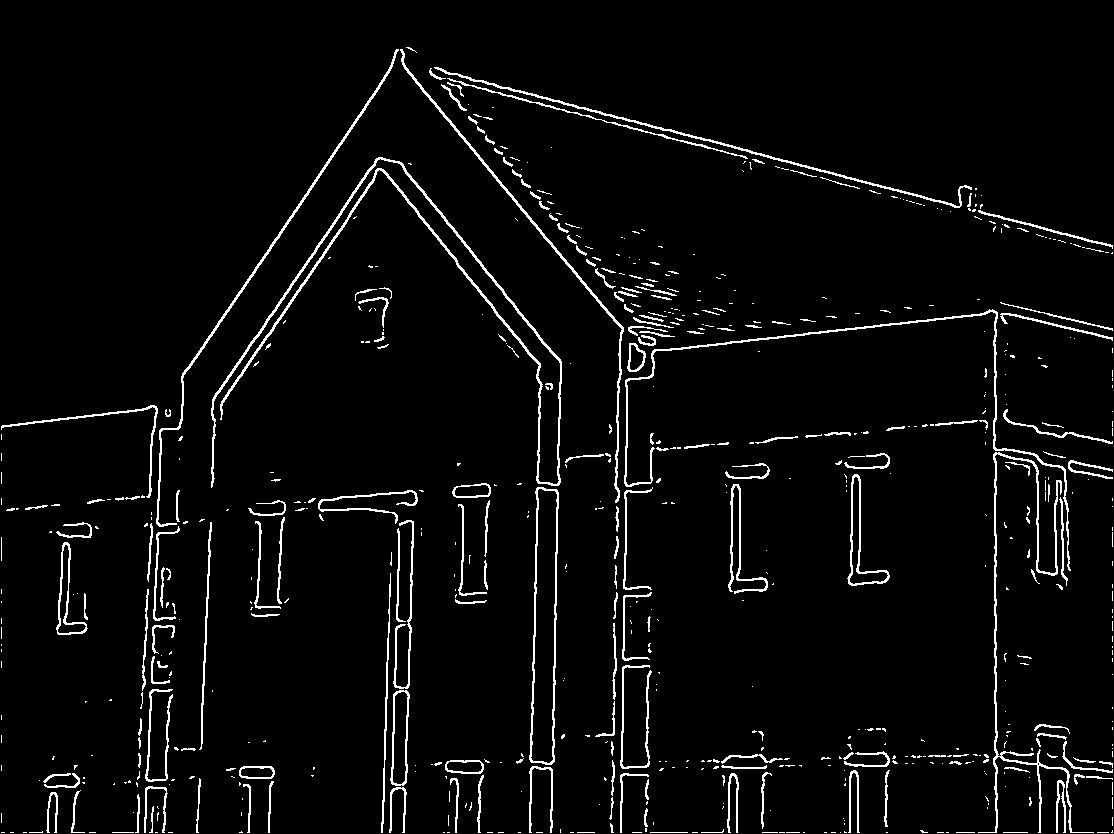
\includegraphics[width=\linewidth]{myfigure/p9/9_zerocross_8.png}
		\caption{}
		\label{fig:zerocross_8}
	\end{subfigure}
	\begin{subfigure}[b]{0.45\linewidth}
		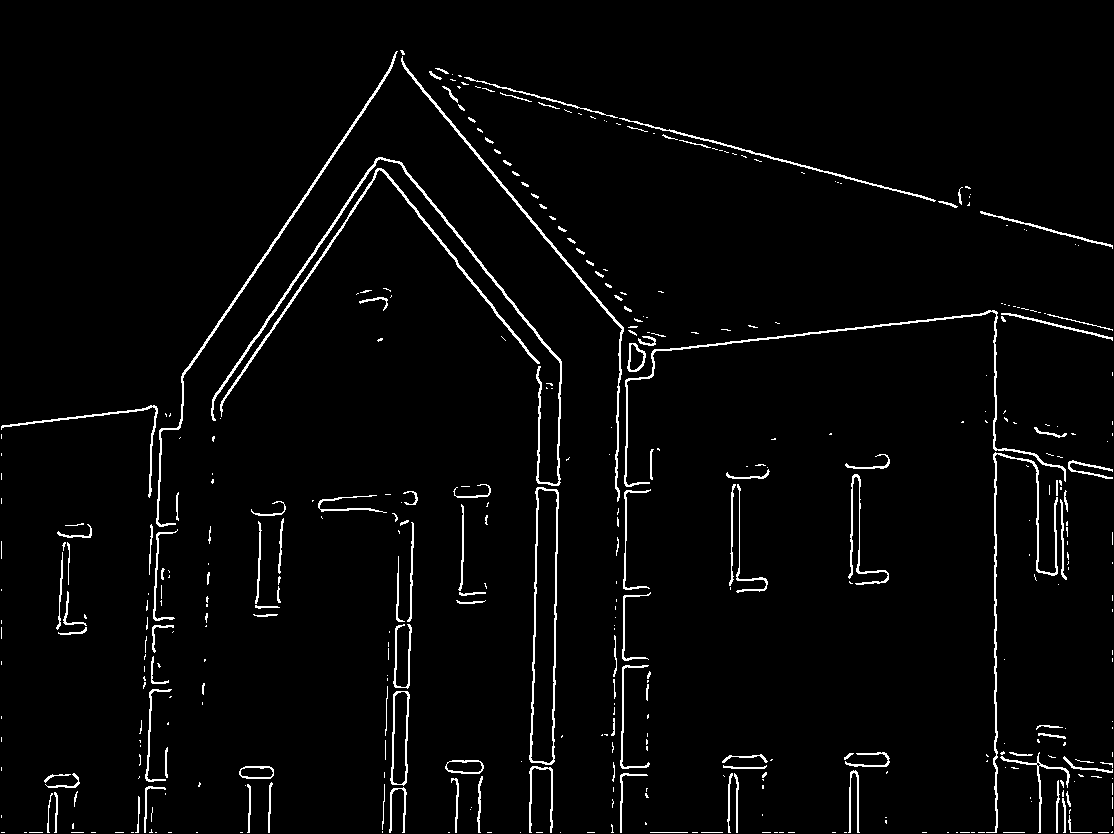
\includegraphics[width=\linewidth]{myfigure/p9/9_zerocross_12.png}
		\caption{}
		\label{fig:zerocross_12}
	\end{subfigure}
	
	\caption{Marr-Hildreth edge detection. \\(a)Original test image of size $834 \times 1115$.\\ (b)Results of Marr-Hildreth(before zero-cross). The gaussian lowpass filter($25\times 25$) used here is with $\sigma=4$.\\  (c)The result of zero cross $threshold=0$.\\ (d)The result of zero cross $threshold=0.04$.\\ (e)The result of zero cross $threshold=0.08$.\\ (f)The result of zero cross $threshold=0.12$.}
  	\label{fig:marr_hildreth}
\end{figure}

Third, I show the process of applying Canny's algorithm in Fig.\ref{fig:eval_canny}. For comparison, Gaussian lowpass filter used here is the same as the one in Marr-Hildreth. The double threshold is $T_H=0.2, T_L=0.1$. We can simply find the Canny's algorithm works better than Marr-Hildreth here. The image in Fig.\ref{fig:thresholdonly} is obtained by use $T_L$, and the result is coarse because of Gaussian smoothing.\\
\begin{figure}[h!]
	\centering
	\begin{subfigure}[b]{0.45\linewidth}
		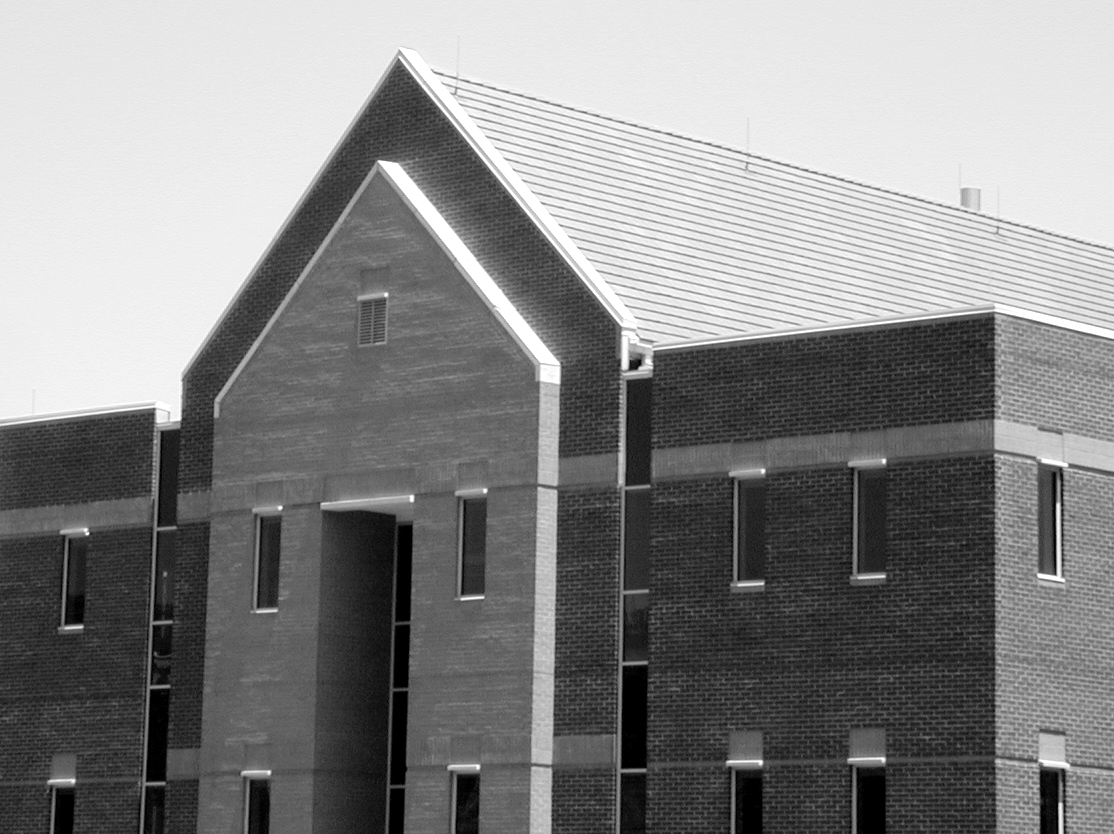
\includegraphics[width=\linewidth]{myfigure/p9/building.png}
		\caption{}
		\label{fig:canny_building}
	\end{subfigure}
	\begin{subfigure}[b]{0.45\linewidth}
    	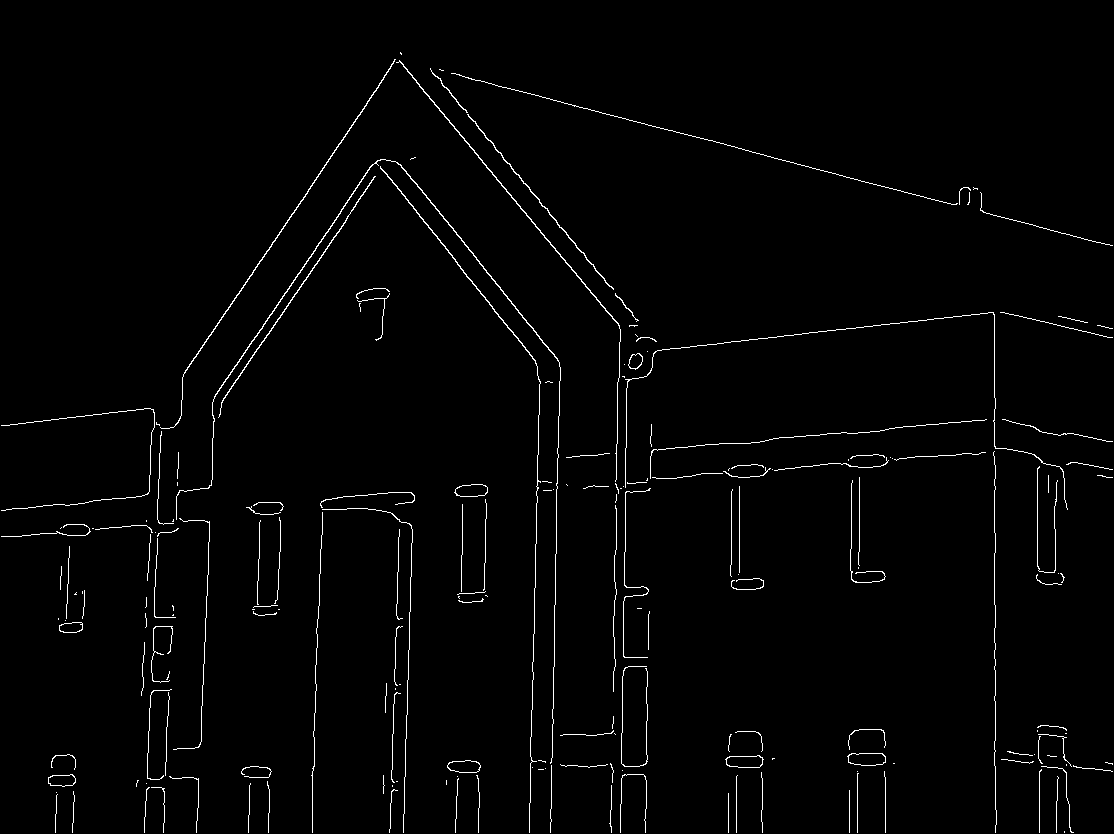
\includegraphics[width=\linewidth]{myfigure/p9/9_threshold_only.png}
    	\caption{}
    	\label{fig:thresholdonly}
  	\end{subfigure}
  	\begin{subfigure}[b]{0.45\linewidth}
		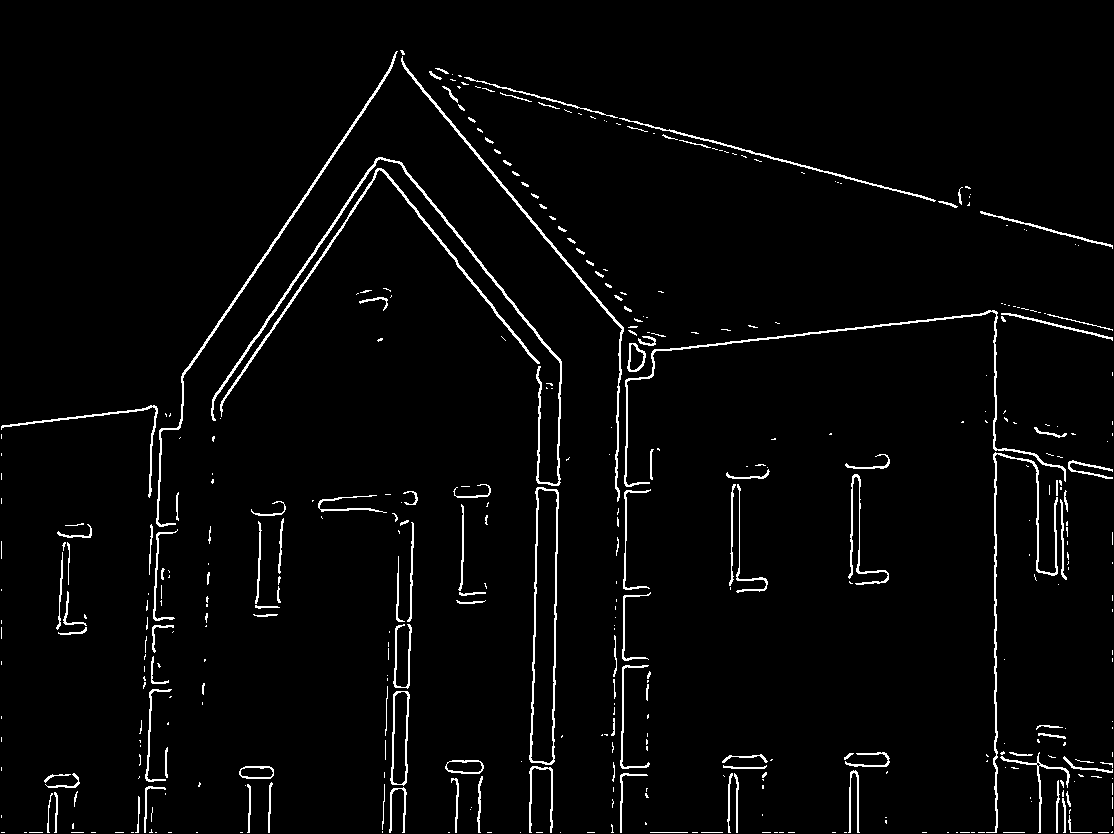
\includegraphics[width=\linewidth]{myfigure/p9/9_zerocross_12.png}
		\caption{}
		\label{fig:zerocross_12_}
	\end{subfigure}
	\begin{subfigure}[b]{0.45\linewidth}
		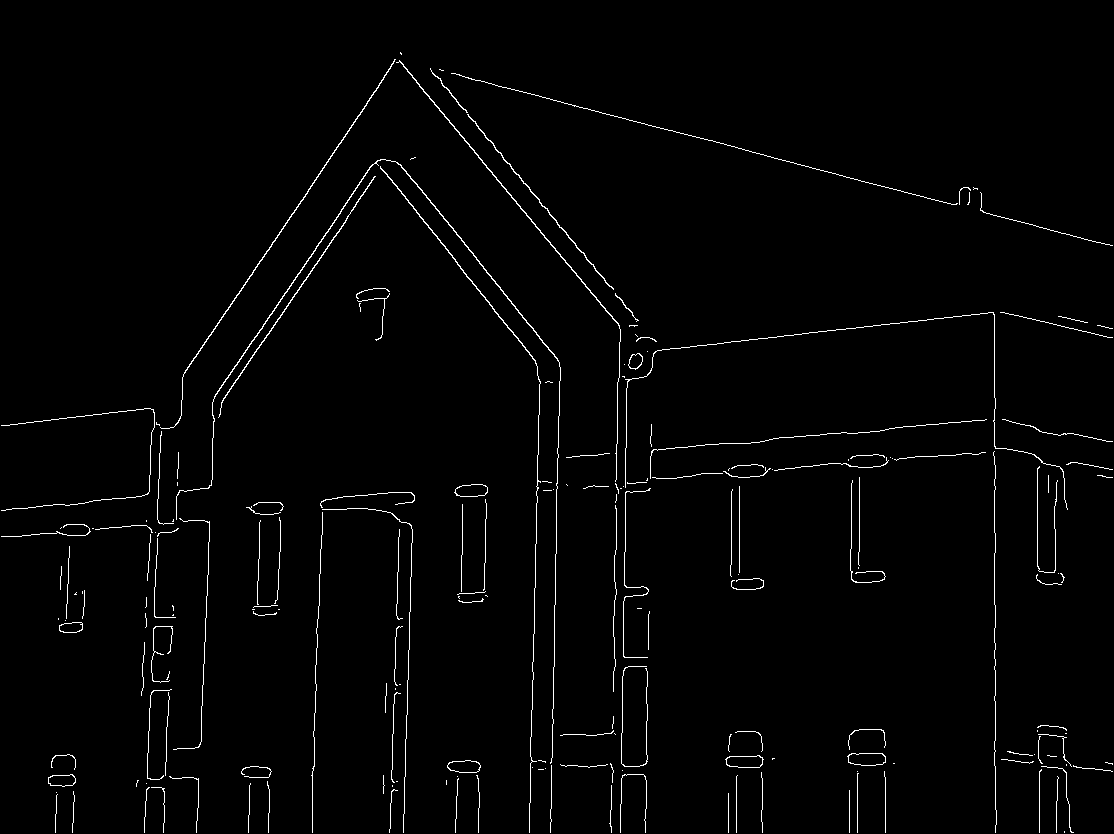
\includegraphics[width=\linewidth]{myfigure/p9/9_canny.png}
		\caption{}
		\label{fig:canny}
	\end{subfigure}
	
	\caption{Canny edge detection. \\(a)Original test image of size $834 \times 1115$.\\ (b)Use single threshold $T_L$ after Gaussian smoothing. \\(c)Result of Marr-Hildreth(before zero-cross). The Gaussian lowpass filter($25\times 25$) used here is with $\sigma=4$.\\ (d)The result of zero cross $threshold=0.04$.}
  	\label{fig:eval_canny}
\end{figure}

\subsubsection{Global thresholding}
Practice on global thresholding is shown in Fig.\ref{fig:globalthresholding}. The original image is an optical microscope image of polymersome cells. From its histogram, we can see the contrast ratio between foreground and background is low. Hence, it's not surprising the basic global thresholding failed. Using Otsu's method here, we obtain good result. In basic thresholding, I set the $\Delta=1.0$, and obtain $T=169.394997$. In Otse's method, the result is $T=181.000000$ and $Seperability=0.465212$. 
\begin{figure}[h!]
	\centering
	\begin{subfigure}[b]{0.45\linewidth}
		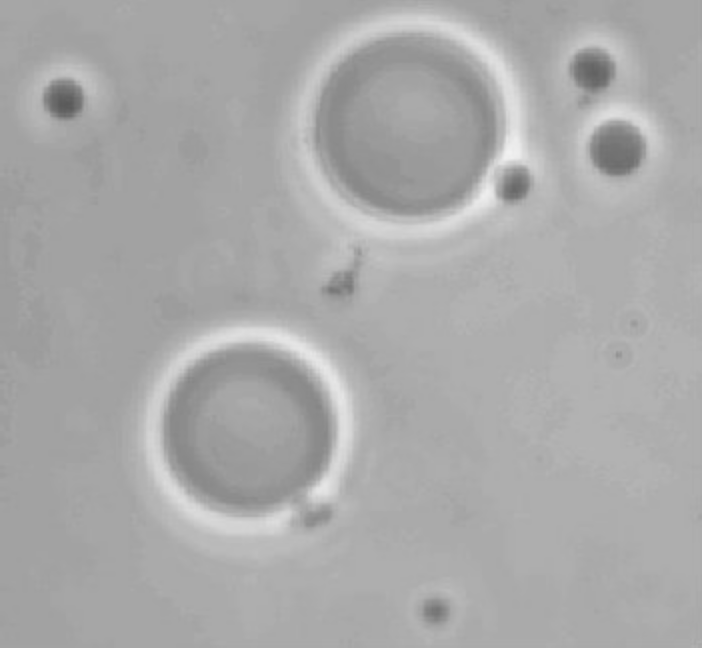
\includegraphics[width=\linewidth]{myfigure/p9/polymersomes.png}
		\caption{}
		\label{fig:polymersomes}
	\end{subfigure}
	\begin{subfigure}[b]{0.45\linewidth}
    	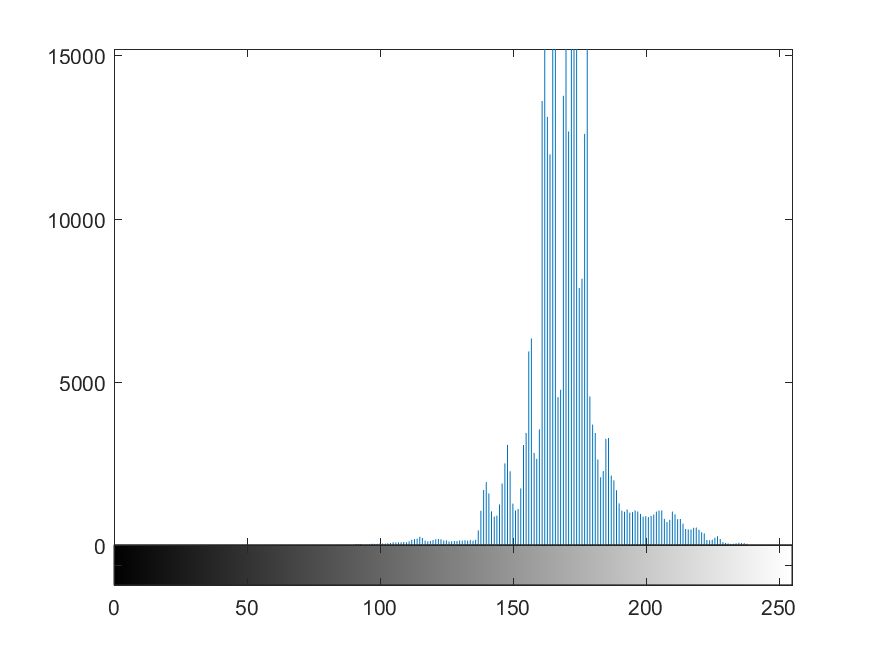
\includegraphics[width=\linewidth]{myfigure/p9/9_polymersomes_hist.png}
    	\caption{}
    	\label{fig:polymersomes_hist}
  	\end{subfigure}
  	\begin{subfigure}[b]{0.45\linewidth}
		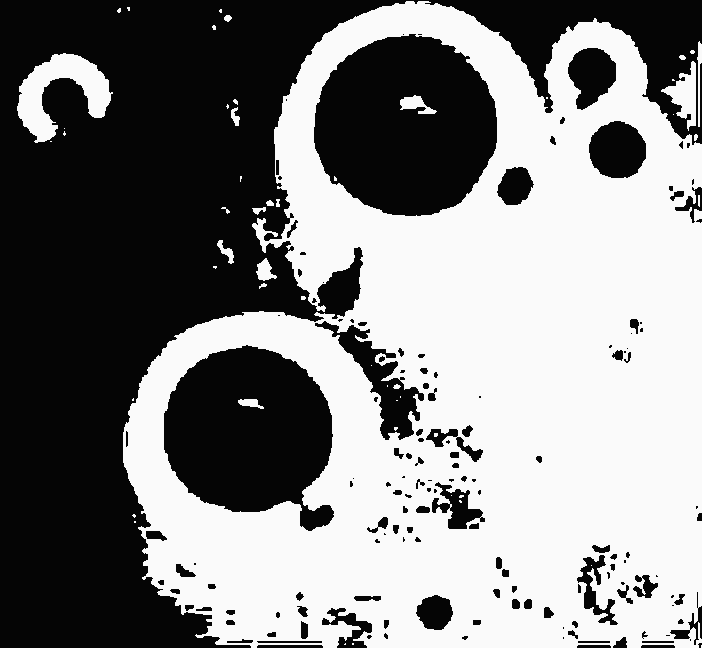
\includegraphics[width=\linewidth]{myfigure/p9/9_threshold_basic.png}
		\caption{}
		\label{fig:threshold_basic}
	\end{subfigure}
	\begin{subfigure}[b]{0.45\linewidth}
		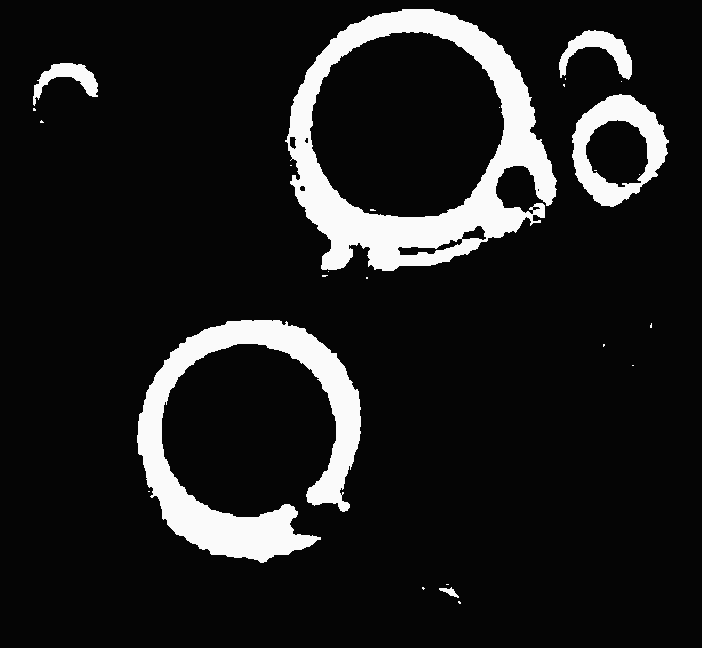
\includegraphics[width=\linewidth]{myfigure/p9/9_threshold_otsu.png}
		\caption{}
		\label{fig:threshold_otsu}
	\end{subfigure}
	
	\caption{Global thresholding. \\(a)Original test image (b)Histogram of the test image. \\(c)Basic thresholding end with $T=169.394997$\\ (d)Otsu's method end with $T=181.000000, sepearablity=0.465212$.}
  	\label{fig:globalthresholding}
\end{figure}

\clearpage
\subsection{Implementation}
Here list the function implemented in this project. They are \emph{roberts, prewitt, sobel, marr\_hildreth, canny, basic\_global\_thresholding, otsu\_thresholding}.

\lstset{language=Matlab}
\begin{lstlisting}
function [ imgg ] = roberts( imgf )
%ROBERTS 
%   robert filter, two with 3x3 masks on axis-x and axis-y

[M, N] = size(imgf);

f = replicate_padding(imgf, 2);
f = double(f); % double f

% Roberts
maskx = [0 0 0 ; 0 -1 0; 0 0 1];
masky = [0 0 0; 0 0 -1; 0 1 0];

gx = zeros(M+4, N+4);
gy = zeros(M+4, N+4);

for x = (2 : M+3)
    for y = (2 : N+3)
        gx(x, y) = sum(sum(f(x-1:x+1, y-1:y+1) .* maskx));
        gy(x, y) = sum(sum(f(x-1:x+1, y-1:y+1) .* masky));
    end
end

% new image: using abs ,some negative
gx = abs(gx(3:M+2, 3:N+2));
gy = abs(gy(3:M+2, 3:N+2));
imgg = scale255(gx+gy);

end
\end{lstlisting}

\lstset{language=Matlab}
\begin{lstlisting}
function [ imgg ] = prewitt( imgf )
%PREWITT prewitt filter
%   two 3x3 masks

[M, N] = size(imgf);

f = replicate_padding(imgf, 2);
f = double(f); % double f

maskx = [-1 -1 -1; 0 0 0; 1 1 1];
masky = [-1 0 1; -1 0 1; -1 0 1];

gx = zeros(M+4, N+4);
gy = zeros(M+4, N+4);

for x = (2 : M+3)
    for y = (2 : N+3)
        gx(x, y) = sum(sum(f(x-1:x+1, y-1:y+1) .* maskx));
        gy(x, y) = sum(sum(f(x-1:x+1, y-1:y+1) .* masky));
    end
end

% new image: using abs ,some negative
gx = abs(gx(3:M+2, 3:N+2));
gy = abs(gy(3:M+2, 3:N+2));
imgg = scale255(gx+gy);

end
\end{lstlisting}
 
 \lstset{language=Matlab}
\begin{lstlisting}
function [ imgg ] = sobel( imgf )
%SOBEL 

[M, N] = size(imgf);

f = replicate_padding(imgf, 2);
f = double(f); % double f

% Sobel
maskx = [-1 -2 -1; 0 0 0; 1 2 1];
masky = [-1 0 1; -2 0 2; -1 0 1];
gx = zeros(M+4, N+4);
gy = zeros(M+4, N+4);
for x = (2 : M+3)
    for y = (2 : N+3)
        gx(x, y) = sum(sum(f(x-1:x+1, y-1:y+1) .* maskx));
        gy(x, y) = sum(sum(f(x-1:x+1, y-1:y+1) .* masky));
    end
end

% new image: using abs
gx = abs(gx(3:M+2, 3:N+2));
gy = abs(gy(3:M+2, 3:N+2));
imgg = scale255(gx+gy);

end
\end{lstlisting}

\lstset{language=Matlab}
\begin{lstlisting}
function [ imgg, imgcross ] = marr_hildreth( imgf, sigma, n, threshold )
%MARR_HILDRETH 
%   sigma - variance of Gaussian, n - size of gaussiain lowpass filter

% generate gaussian filter
x = (1:n) - (n+1)/2;
y = x';
x = repmat(x, n, 1);
y = repmat(y, 1, n);
D2 = x.^2 + y.^2;
gau_filter = exp(-D2 / (2*sigma*sigma));

% preprocess
[M, N] = size(imgf);
imgf = double(imgf) ./ 255;
f = replicate_padding(imgf, n-1);
f = double(f); % double f

% convolution
g = zeros(M+2*n, N+2*n);
for x = (n : M+n-1)
    for y = (n : N+n-1)
        xlow = fix(x - fix((n-1)/2));
        xhigh = fix(x + fix((n-1)/2));
        ylow = fix(y - fix((n-1)/2));
        yhigh = fix(y + fix((n-1)/2));
        g(x,y) = sum(sum(f(xlow:xhigh,ylow:yhigh) .* gau_filter));
    end
end

f = g(n:M+n-1, n:N+n-1) * 255;
% laplacian
f = replicate_padding(f, 2);
mask = [1 1 1; 1 -8 1; 1 1 1];
g = zeros(M+4, N+4);
for x = (2 : M+3)
    for y = (2 : N+3)
        g(x, y) = sum(sum(f(x-1:x+1, y-1:y+1) .* mask));
    end
end

% do zero cross
g = g(3:M+2, 3:N+2);
imgcross = zero_cross(g, threshold*max(max(g)));

imgg = g; % laplacian result without scale
imgg = scale255(imgg); % this is the image to show
imgcross = scale255(imgcross);

end
\end{lstlisting}

\lstset{language=Matlab}
\begin{lstlisting}
function [ imgg, imgt ] = canny( imgf, sigma, n, TL, TH )
%CANNY canny's algorithm
%   sigma - gaussian variance, n - size of filter, TH TL - thresholds

% generate gaussian filter
x = (1:n) - (n+1)/2;
y = x';
x = repmat(x, n, 1);
y = repmat(y, 1, n);
D2 = x.^2 + y.^2;
gau_filter = exp(-D2 / (2*sigma*sigma));

% preprocess
[M, N] = size(imgf);
imgf = double(imgf) ./ 255;
f = replicate_padding(imgf, n-1);
f = double(f); % double f

% gaussian smoothing
g = zeros(M+2*n, N+2*n);
for x = (n : M+n-1)
    for y = (n : N+n-1)
        xlow = fix(x - fix((n-1)/2));
        xhigh = fix(x + fix((n-1)/2));
        ylow = fix(y - fix((n-1)/2));
        yhigh = fix(y + fix((n-1)/2));
        g(x,y) = sum(sum(f(xlow:xhigh,ylow:yhigh) .* gau_filter));
    end
end

% restore to original size
f = g(n:M+n-1, n:N+n-1);
minf = min(min(f));
maxf = max(max(f));
f = (f - minf)./(maxf-minf); % normalization to (0,1)

% calculate magnitude and angle image
magnitude = zeros(M, N);
angle = zeros(M, N);
for x = (1:M-1)
    for y = (1:N-1)
        py = f(x,y) - f(x,y+1) + f(x+1,y) - f(x+1,y+1);
        px = f(x,y) - f(x+1,y) + f(x,y+1) - f(x+1,y+1);
        magnitude(x, y) = sqrt(px*px + py*py);
        angle(x, y) = atand(py/px);
    end
end

% obtain thresholding-only image
imgt = zeros(M, N);
for x = (1:M)
    for y = (1:N)
        if magnitude(x,y)>=TL 
            imgt(x,y) = magnitude(x,y);
        end
    end
end
imgt = uint8(scale255(imgt));

% nonmaximum suppression
suppres = zeros(M, N);

for x = (2:M-1)
    for y = (2:N-1)
        if angle(x,y)>=-22.5 && angle(x,y)<22.5 % horizontal
            if magnitude(x,y)>magnitude(x-1,y) && magnitude(x,y)>magnitude(x+1,y)
                suppres(x, y) = magnitude(x,y);
            end
        elseif angle(x,y)>=22.5 && angle(x,y)<67.5 % leftbottom-righttop
            if magnitude(x,y)>magnitude(x-1,y-1) && magnitude(x,y)>magnitude(x+1,y+1)
                suppres(x, y) = magnitude(x,y);
            end
        elseif angle(x,y)>=-67.5 && angle(x,y)<-22.5 % lefttop-rightbottom
            if magnitude(x,y)>magnitude(x-1,y+1) && magnitude(x,y)>magnitude(x+1,y-1)
                suppres(x, y) = magnitude(x,y);
            end
        else % vertical
            if magnitude(x,y)>magnitude(x,y+1) && magnitude(x,y)>magnitude(x,y-1)
                suppres(x, y) = magnitude(x,y);
            end
        end
    end
end

% double thresholding
imgg = zeros(M, N);

for x = (1:M)
    for y = (1:N)
        if suppres(x,y)>TH % strong edge pixel
            imgg(x,y) = 1;
        elseif suppres(x,y)>TL 
            if max(max(suppres(x-1:x+1,y-1:y+1)))>TH % 8-connectivity
                imgg(x,y) = 1;
            end
        end            
    end
end

end
\end{lstlisting}

\lstset{language=Matlab}
\begin{lstlisting}
function [ imgg, T ] = basic_global_thresholding( imgf, T0, deltaT )
%BASIC_GLOBAL_THRESHOLDING 
%   T0: init esitimatation threshold, deltaT: the stopping difference

while 1
    [~, mean_0, mean_1] = thresholding(imgf, T0);
    T1 = (mean_0+mean_1)/2;
    if abs(T1-T0) <= deltaT
        T = T1;
        break
    end
    T0 = T1;
end
[imgg, ~, ~] = thresholding(imgf, T);

end

function [ imgg, mean_0, mean_1 ] = thresholding( imgf, T )    
[M, N] = size(imgf);
imgg = zeros(M, N);
mean_0 = double(0);
mean_1 = double(0);
cnt_0 = 0;
cnt_1 = 0;
for x = (1:M)
    for y = (1:N)
        if imgf(x,y)>T
            imgg(x,y)=250;
            mean_1 = mean_1+double(imgf(x,y));
            cnt_1 = cnt_1+1;
        else
            imgg(x,y)=5;
            mean_0 = mean_0+double(imgf(x,y));
            cnt_0 = cnt_0+1;
        end
    end
end

imgg = uint8(imgg);
if mean_0 == 0
    cnt_0 = 1;
end
if mean_1 == 0
    cnt_1 = 1;
end

mean_0 = mean_0 / cnt_0;
mean_1 = mean_1 / cnt_1;

end
\end{lstlisting}

\lstset{language=Matlab}
\begin{lstlisting}
function [ imgg, kstar, eta ] = otsu_thresholding( imgf )
%OTSU_THRESHOLDING 
%   kstar: threshold, eta: separability

[M, N] = size(imgf);
histf = zeros(1, uint32(256)); % (0:255)
for x=(1:M)
    for y=(1:N)
        histf(fix(imgf(x,y)+1)) = histf(fix(imgf(x,y)+1)) + 1;
    end
end
histf = double(histf)/double(M*N);

P = zeros(1, uint32(256));
P(1) = histf(1);
for i = (2:256)
    P(i) = P(i-1) + histf(i);
end

m = double(zeros(1, uint32(256)));
m(1) = 0*double(histf(1));
for i = (2:256)
    m(i) = m(i-1) + double(i-1)*histf(i);
end
mG = m(256);

size(P)
size(m)
size(mG)
size(1-P)

sigmaB2 = (mG .* P - m) .^2 ./(P .* (1-P));
size(sigmaB2)
kall = find(sigmaB2==max(sigmaB2));
kstar = mean(kall) - 1;
sigmaG = sum(((0:255)-mG).^2 .* histf);

eta = sigmaB2(int32(kstar)) / sigmaG;
imgg = thresholding(imgf, kstar);

end

function [ imgg ] = thresholding( imgf, T )    
[M, N] = size(imgf);
imgg = zeros(M, N);
for x = (1:M)
    for y = (1:N)
        if imgf(x,y)>T
            imgg(x,y)=250;
        else
            imgg(x,y)=5;
        end
    end
end

imgg = uint8(imgg);
end
\end{lstlisting}

